\documentclass[letterpaper, 12pt]{article}
\usepackage[]{graphicx}
\usepackage[]{color} % use "amsart" instead of "article" for AMSLaTeX format
\usepackage{geometry}                % See geometry.pdf to learn the layout options. There are lots.
\geometry{letterpaper}                     % ... or a4paper or a5paper or ... 
\usepackage{apacite}
%\usepackage{subfigure}
%\usepackage{alltt}
%\usepackage{etex}     
%\usepackage{amsfonts, amsmath, amssymb, latexsym, mathrsfs, fancyhdr,theorem,  pifont, setspace, verbatim,  qtree, lscape, tipa, linguex, hyperref, wasysym, stmaryrd, natbib,soul, minibox, lipsum, setspace, amssymb, color, multirow, multicol, soul,geometry,graphicx, wrapfig,gb4e,booktabs}
%\usepackage[T1]{fontenc}
%\usepackage{times}
%\usepackage{helvet}
%\renewcommand{\familydefault}{\sfdefault}
\geometry{hmargin={1in,1in},vmargin={1in,1in}}
\definecolor{Red}{RGB}{255,0,0}
\graphicspath{{../cogsci2019/figs/}}

\newcommand{\denote}[1]{\mbox{ $[\![ #1 ]\!]$}}
\usepackage{tikz}
\usepackage{tikz-qtree}
\usepackage{caption}
\usepackage{wrapfig}
\usepackage{pslatex}
\usepackage{apacite}
\usepackage{amsmath}
\usepackage{float} % Roger Levy added this and changed figure/table
                   % placement to [H] for conformity to Word template,
                   % though floating tables and figures to top is
                   % still generally recommended!

%\title{Brief Article}
%\author{Authors}
%\date{ % Activate to display a given date or no date


\begin{document}
\begin{center}
\textbf{Incremental understanding of conjunctive generic sentences}
\end{center}

Generic statements convey generalizations about categories, but how generic predications should combine is unclear.
``Elephants live in Africa and Asia'' does not mean that individual elephants live on both continents; instead, the sentence should be understood as \emph{elephants live in Africa, and elephants live in Asia}, but this is impossible if each individual generic sentence means that the majority hold the property \cite<i.e., it is impossible for more than half of elephants to live in Africa and more than half of elephants to live in Asia;>{Nickel2008}.  
%In this case, the \emph{prevalence} required for endorsing a generic involving a conjunctive predication seems more lax than if only one of conjuncts were mentioned: ``Wugs live in Africa'' intuitively still conveys that most or all wugs live in Africa.
The puzzle of understanding conjunctive generic sentences deepens when one considers that actual linguistic input is processed incrementally: Listeners ubiquitously form expectations about the intended meaning before the speaker finishes their sentence \cite<e.g.,>{tanenhaus1995integration}.  For conjunctive generics about mutually exclusive (ME) properties, strongly incremental language understanding might produce non-monotonic interpretation updates: after the sentence prefix ``Elephants live in Africa\ldots'', a comprehender might infer a higher property \emph{prevalence} than after hearing the sentence completion ``\ldots and Asia''. 
%If such non-monotonic updates occur, what types of linguistic input trigger them?  

\begin{wrapfigure}{r}{0.4\textwidth}
\vspace{-1cm}
  \begin{center}
    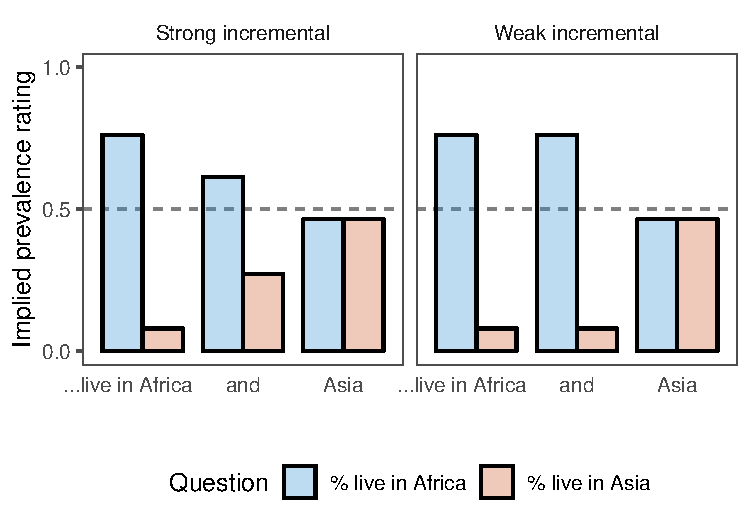
\includegraphics[width=0.4\textwidth]{incremental}
  \end{center}
  \vspace{-0.45cm}
  \caption{\small A model that incorporates syntactic expectations at the level of individual words predicts intermediate mutual-exclusivity inferences part-way through the conjunction (at ``and''), whereas a model that waits for content-words (e.g., ``Asia'') to begin to understand the utterances does not show a difference in expected prevalence at the word ``and.''}
  \label{fig:incremental}
\end{wrapfigure}


To explore the implications of these ideas, we extend a model for interpreting generic language to incorporate an incremental processing mechanism that allows a listener to understand partial utterances.
The original model of \citeA{Tessler2019:genLang} can already adjust the meaning of a generic utterance by reasoning about an underspecified threshold $\theta$.
To interpret a generic about a conjunctive predicate such as ``Elephants live in Africa and Asia'', we assume the sentence gets parsed into: $[G_\theta x. \textnormal{ elephants}(x) \to \textnormal{live\_in}(\textnormal{Africa})] \land [G_\theta x. \textnormal{ elephants}(x) \to \textnormal{live\_in}(\textnormal{Asia})]$ (see \citeA{Nickel2008} for supporting arguments).
The model can then interpret multiple generics in succession, using the posterior distribution over prevalence as the prior for the next utterance. 
The model makes the prediction that for ME properties, conjunctive generics will non-monotonically update beliefs about the property prevalence in the target category. 

If listeners parse and interpret utterances incrementally at the level of individual words, then incorporating probabilistic syntactic expectations \cite{Levy2008} into this model predicts that when a comprehender encounters the conjunction ``and'', they will infer the prevalence of elephants in Africa as a mixture of the inferences derived from different possible continuations (e.g., if the full sentence will be ``live in Africa and eat bugs''~vs.~``live in Africa and Asia'').
If, however, listeners do not derive incremental interpretations at each moment, but instead wait for meaningful pieces of an utterance (e.g., content words like \emph{Asia}) to compute interpretations, then we would not expect such an intermediate degree of interpretation: ``Elephants live in Africa and\ldots'' should mean the same thing as ``Elephants live in Africa\ldots'' (Fig.~\ref{fig:incremental}). 

%When processing a conjunctive phrase, listeners may form expectations about the complete utterance even before the sentence is over. 
%For example, when a speaker reaches the word \emph{and} in ``Elephants live in Africa \emph{and}'', she has two syntactically distinct options available to her when completing the sentence: She could continue with a noun phrase (e.g., ``and Asia'') or a verb phrase (e.g., ``and eat bugs'').
%Each of these continuations would imply different inferences about the prevalence of elephants in Africa.\footnote{
%	Of course, it is possible to continue with a verb phrase about a mutually exclusive property such as ``\ldots live in Africa and live in Asia'' as well as continue with a noun phrase about a non-mutually exclusive property (e.g., ``\ldots eat figs and nuts''). Our focus is on the fact that a speaker can continue the conjunction with a mutually exclusive or non-mutually exclusive property, which in the cases we consider, are highly correlated with NP~vs.~VP coordination.
%}
%If listeners parse and interpret utterances incrementally at the level of individual words, then we would expect their 

\begin{figure}[t]
%\vspace{-1cm}
  \begin{center}
    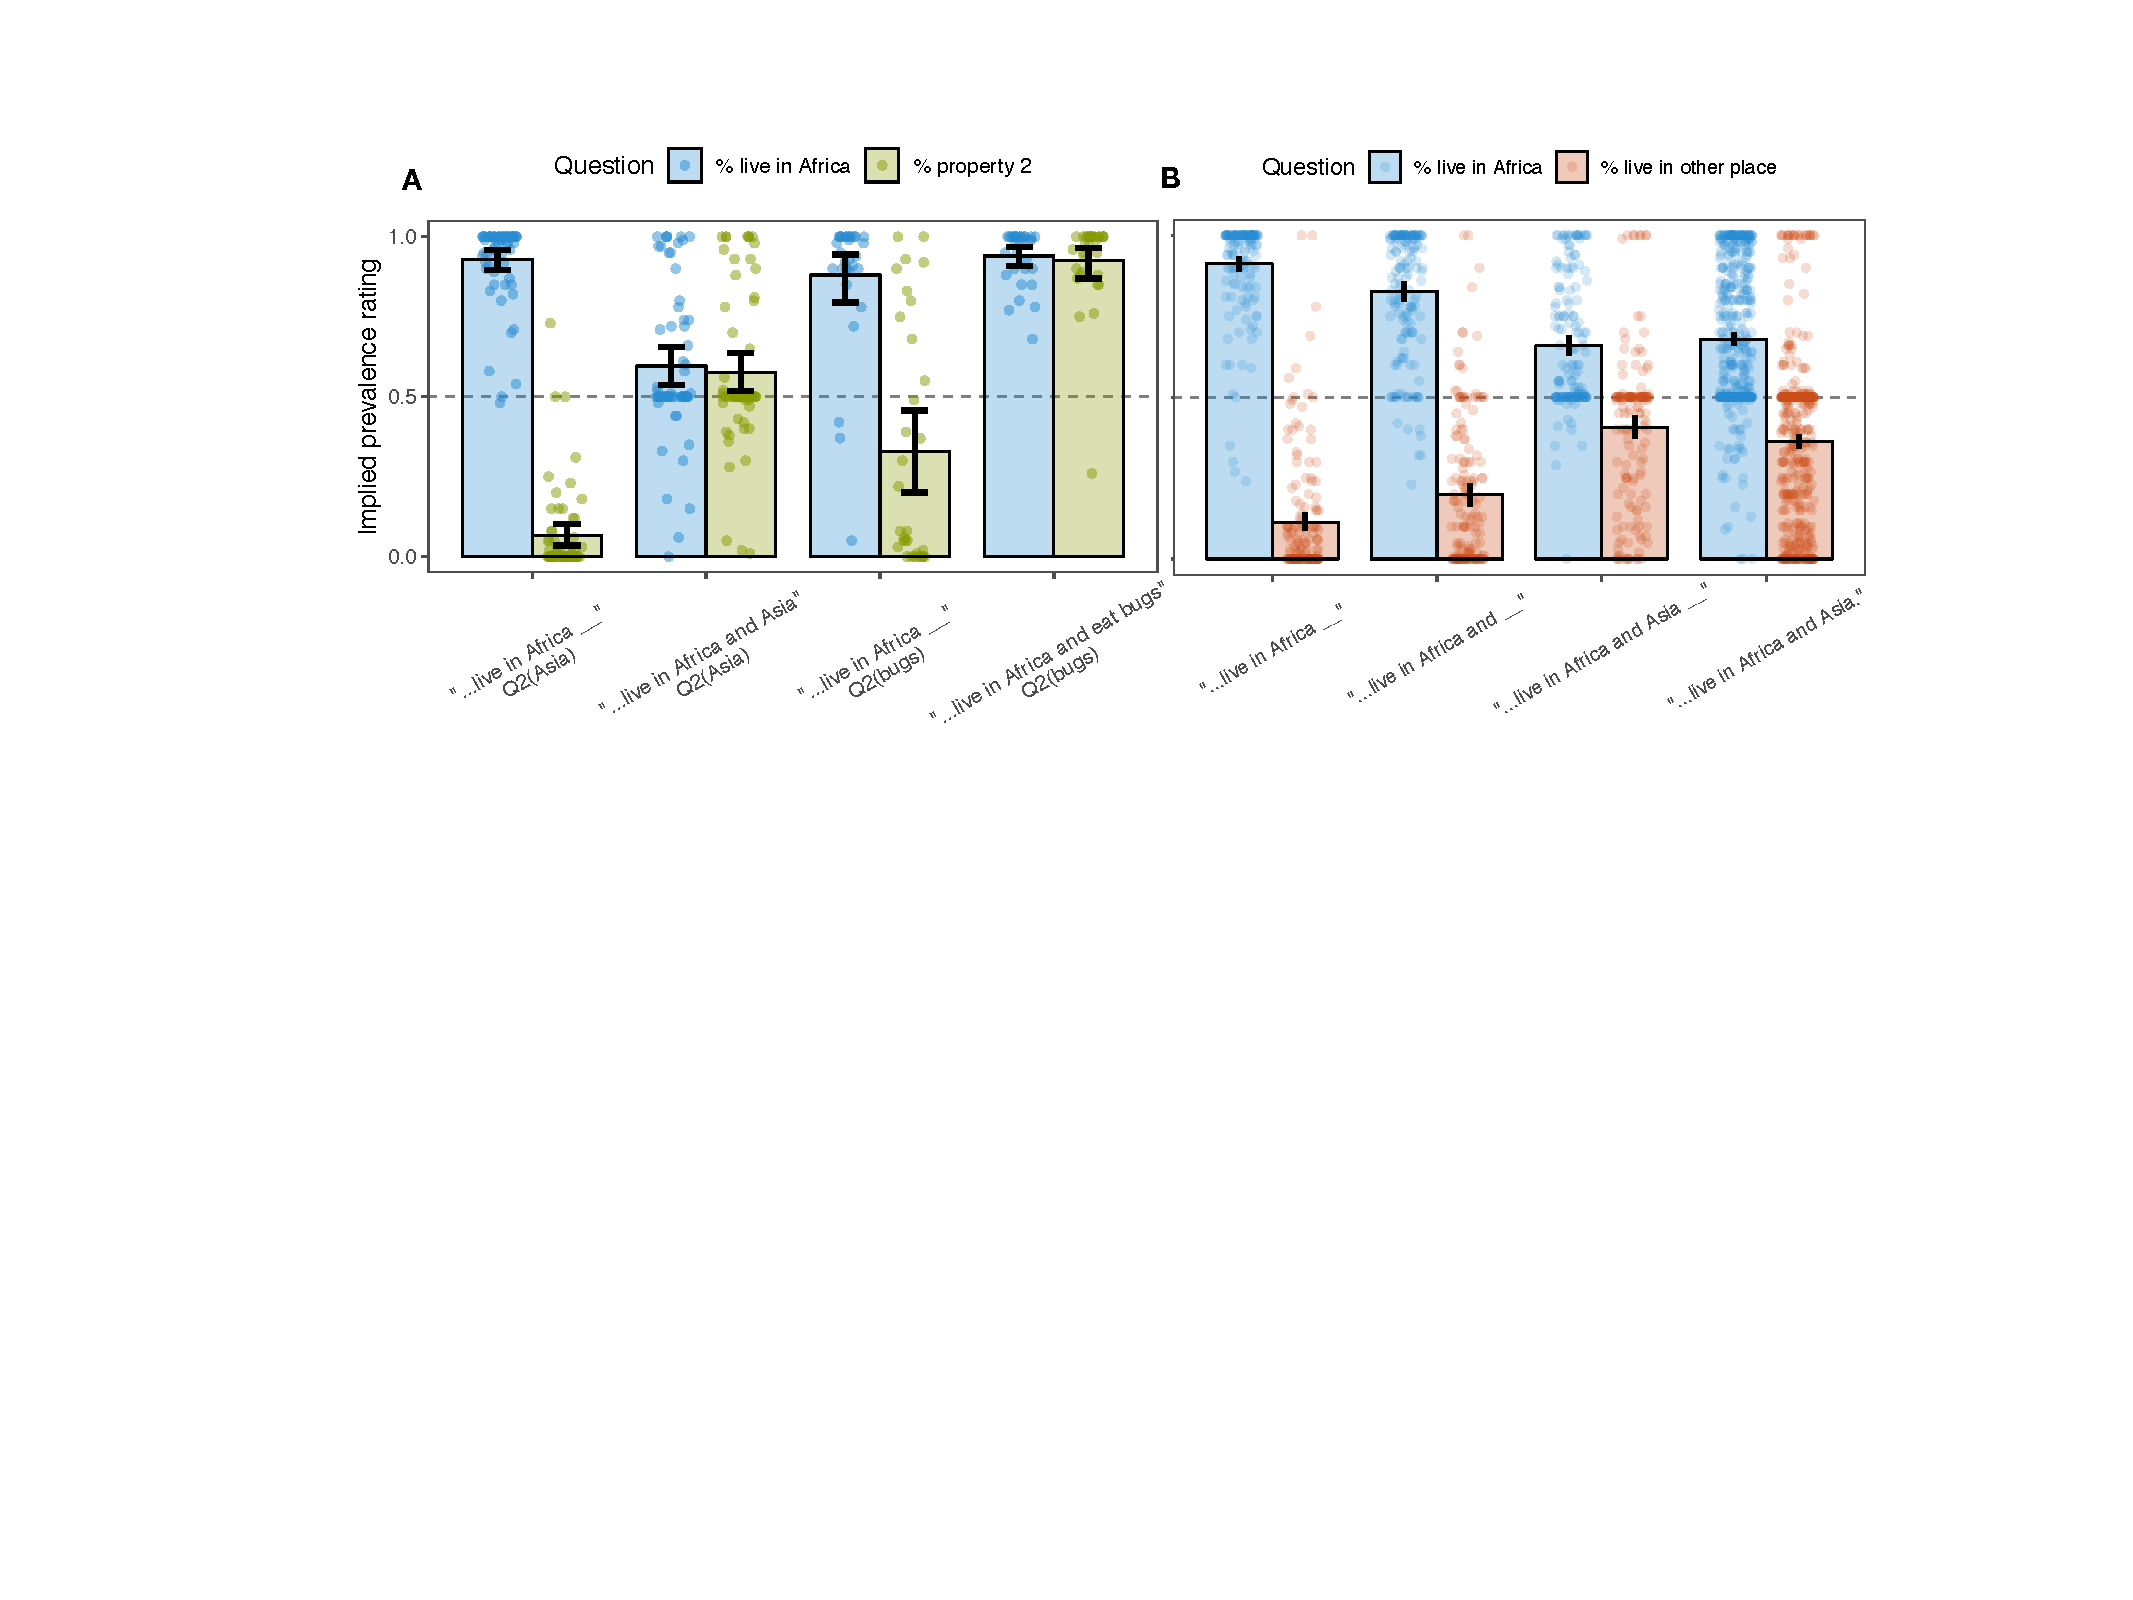
\includegraphics[width=0.9\textwidth]{xprag}
  \end{center}
  \vspace{-0.55cm}
  \caption{\small Experimental results. A: Participants rate prevalence for mentioned property (\% live in Africa) and ``Property 2'', either the mutually exclusive property (left two bars) or non-mutually exclusive property (right two bars).  B: Participants are interrupted at various stages of the sentence (either after \emph{Africa}, \emph{and}, or \emph{Asia}) to be asked about the prevalence of \emph{living in Africa} and \emph{living in some other place}, or asked at the end of the sentence (right-most bars). ``\_\_'' indicates the question appears mid-sentence. Error-bars denote bootstrapped 95\% confidence intervals.}
  \label{fig:results}
    \vspace{-0.55cm}
\end{figure}

We design two experiments to test the mutual exclusivity (ME) and incremental predictions of the model. 
The first experiment tests the ME predictions that ``Elephants live in Africa and Asia'' means roughly that half live in Africa and half live in Asia.%; this experiment also serves to validate the gating procedure we employ in the second experiment. 
The second experiment is a pre-registered study that uses the gating paradigm to test the fine-grained incremental predictions of the model.
The experiments and list of materials can be viewed at \url{tinyurl.com/elephants-cogsci}.

%\begin{wrapfigure}{r}{0.5\textwidth}
%\vspace{-1cm}
%  \begin{center}
%    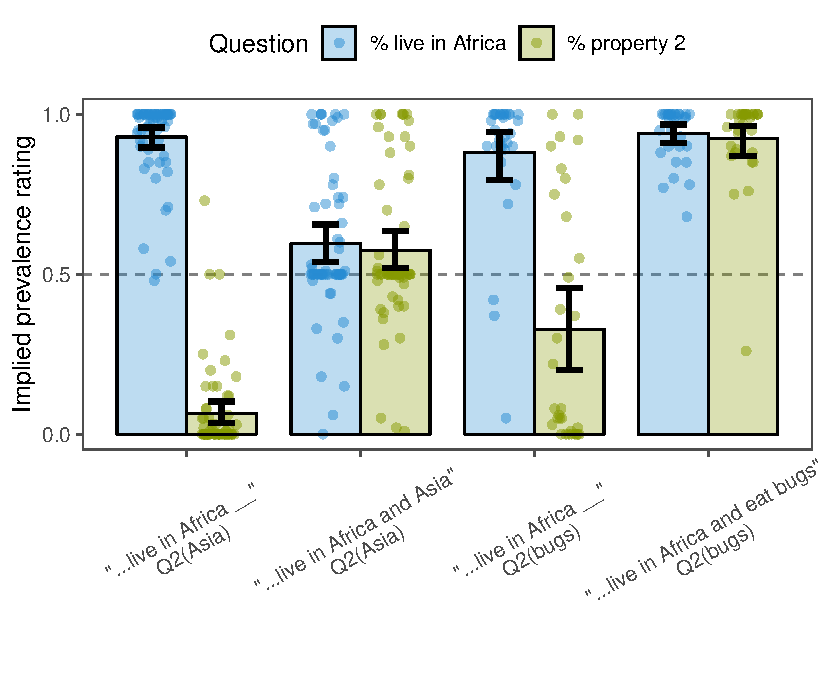
\includegraphics[width=0.48\textwidth]{expt2_summary}
%  \end{center}
%  \vspace{-1cm}
%  \caption{\small Experiment 1 results.  Participants rate prevalence for mentioned property (\% live in Africa) and ``Property 2'', either the mutually exclusive property (left two bars) or non-mutually exclusive property (right two bars). ``\_\_'' indicates the question appears mid-sentence. Error-bars denote bootstrapped 95\% confidence intervals.}
%  \label{fig:expt1}
%\end{wrapfigure}

In both experiments, participants read a storybook about creatures on a faraway planet. Chapters of the book consist of a few sentences teaching about the category. Critical trials end with a conjunctive generic sentence (``Ks F and G''). Participants are asked to rate the \% of Ks with F and the \% of Ks with G using two slider bars ranging from 0\% to 100\%. Filler trials contain sentences using quantifiers \emph{all}, \emph{most}, and \emph{none}.% and participants are asked to rate the prevalence of the properties described with quantifiers. 

Expt. 1 contains four conditions, which are randomized within-participant and within-item. In two of the conditions, participants are asked about two ME properties (e.g., living in Africa and Asia); in the other two, participants are asked about two non-ME (NME) properties (e.g., living in Africa and eating bugs). For each of these conditions, participants are either asked at the end of the chapter (i.e., after the full conjunctive generic) or before the final page of the chapter, where the conjunctive generic is broken before the ``and'' (i.e., participants only read ``Elephants live in Africa'' and are asked the question mid-sentence). We find that when asked about mutually exclusive properties, participants exhibit non-monotonic belief updating, first believing that almost all elephants live in Africa and then believing that only half life in Africa; this phenomenon is not observed when asking about non-mutually properties predicated of a category (Fig.~\ref{fig:results}A).

%\begin{wrapfigure}{l}{0.5\textwidth}
%\vspace{-1cm}
%  \begin{center}
%    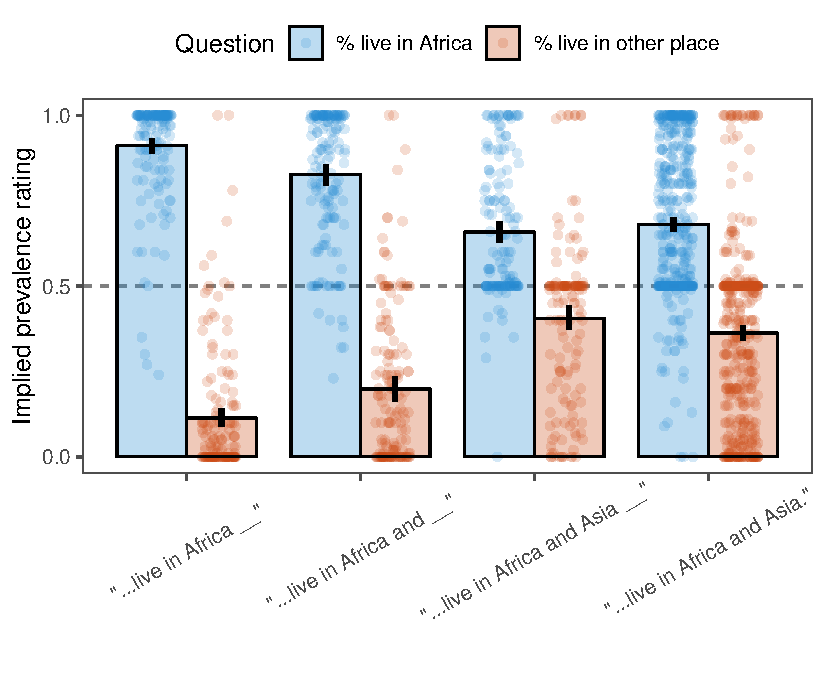
\includegraphics[width=0.48\textwidth]{expt3_summary}
%  \end{center}
%  \caption{\small Experiment 2 results. Participants are interrupted at various stages of the sentence (either after \emph{Africa}, \emph{and}, or \emph{Asia}) to be asked about the prevalence of \emph{living in Africa} and \emph{living in some other place}, or asked at the end of the sentence (right-most bars). When participants are interrupted before the second conjunct (\emph{Asia}), the sentence continues with a non-mutually exclusive property. Error-bars denote bootstrapped 95\% confidence intervals.
%}
%\vspace{-1cm}
%\label{fig:expt2}
%\end{wrapfigure}




Having validated the method, we aimed to test the incremental prediction of the model that when participants only hear ``Elephants live in Africa and'', they will begin to anticipate a mutually-exclusive conjunct, and that this would manifest in their implied prevalence ratings being substantially less than when they only hear ``Elephants live in Africa''.
Expt.~2 contained three conditions, corresponding to the point in the conjunctive generic sentence at which the page-break and prevalence questions occurred: ``Elephants live in Africa\_\_ and\_\_ Asia\_\_'' (where \_\_ denotes the point at which the page broke and the prevalence questions were presented).
In a pre-registered study, we found that participants provided substantially lower estimates of prevalence when provided with the conjunct ``and'' in a partial sentence (posterior mean estimate and 95\% credible interval: $\beta = -0.08 (-0.13, -0.04)$) and that these ratings were also substantially higher than when participants read the full conjunctive predicate ($\beta = 0.17 (0.12, 0.23)$; Fig.~\ref{fig:results}B). 
These results support a strong view of incrementality, suggesting that listeners begin to draw pragmatic interpretations of generics before the end of the sentence and even in the absence of additional content words. 








\bibliographystyle{apacite}

\setlength{\bibleftmargin}{.125in}
\setlength{\bibindent}{-\bibleftmargin}

\bibliography{../cogsci2019/elephants}
\renewcommand\bibname{}
\scriptsize
%Extending an analysis of generics to handle complex-predicates poses unique challenges.
%A sentence of the form ``Ks F and G'' introduces an ambiguity:
%
%\begin{enumerate}
%\tightlist
%\item $\denote{gen}(K) [F \land G]$
%\item $\denote{gen}(K) [F] \land \denote{gen}(K) [G]$
%\end{enumerate}


\end{document}
